
\section{OpenRefine}
%------------------------------------------------------------------------------
\begin{frame}[allowframebreaks]{Wozu OpenRefine?}
 \metroset{block=fill}
 
\begin{columns}
  \column{0.45\textwidth}
  \begin{block}{OpenRefine nutzen}\footnotesize 
  Könnte eine Ressource sein, die Sie zur Befüllung Ihrer Datenbank / Datenakquise nutzen.
Man kann damit 
\begin{itemize}
    \item Daten aus dem Internet ziehen (\alert{Web Scraping})
    \item Daten bereinigen, also z.B. Inkonsistenzen bereinigen, mehrere Werte in Einzelzellen auftrennen, Duplikate entfernen, aber auch analyisieren. 
\end{itemize}
\end{block}

  \column{0.55\textwidth}
\begin{alertblock}{\small Messy Data bereinigen mit OpenRefine}
  \begin{enumerate}\footnotesize 
    \item ursprünglich von Google entwickelt 
    \item mittlerweile Open Source Projekt 
    \item mächtige Filterungsmöglichkeiten
    \item Datentransformationen können gespeichert werden und auf andere Datensets angewendet werden 
    \item vor allem für Daten in Tabellenform
    \item GREL (\emph{General Refine Expression Language}) Sprache zur Datentransformation
 \end{enumerate}
%Jython (Jython = implementation of Python on JVM)
\end{alertblock}
\end{columns}
\end{frame}

%------------------------------------------------------------------------------

\begin{frame}{OpenRefine}
    \begin{quote}
        OpenRefine is a powerful, free and open source tool that can be used for data cleaning.
        
        OpenRefine will automatically track any steps allowing you to backtrack as needed and providing a record of all work done
    \end{quote}
    % ----------------------------------------------
  \begin{columns}[T,onlytextwidth]
  \metroset{block=fill}
    \column{0.45\textwidth}


      \begin{block}{Datenbereinigung}\footnotesize 
Entfernen und Ausbessern von Datenfehlern in Datenbanken, Tabellen etc. 
Unvollständige, fehlerhafte, unpräzise, irrelevante, überflüssige Daten (= “schmutzige Daten”) verändern, ersetzen oder löschen. 
      \end{block}

      \begin{block}{Datenintegration}\footnotesize 
Daten aus mehreren Quellen mit einander verschmelzen,
um konsistente Daten zu erhalten. 
      \end{block}
    % ----------------------------------------------
    \column{0.45\textwidth}

      \metroset{block=fill}

      \begin{block}{Data Transformation}\footnotesize 
      Rohdaten (\emph{raw data}) werden in ein nützliches Format konvertiert; Daten werden aggregiert, d.h. zusammengeführt. 
      \end{block}
      
      \begin{block}{(Data Reduction)}\footnotesize 
      Kompression der Daten hinsichtlich nützlicher Werte (Entfernen irrelevanter Informationen); Verbesserung der Effizienz der Organisation, z.B. zum Sortieren, etc.
      \end{block}
      
  \end{columns}
\end{frame}

%------------------------------------------------------------------------------
\begin{frame}[fragile,allowframebreaks]{Daten bereinigen}
 \metroset{block=fill}
 
\begin{columns}
  \column{0.55\textwidth}
\begin{block}{Typische Anwendungen der GREL}
\begin{enumerate}\footnotesize
    \item Common usage: \texttt{value.toUppercase(); value.toLowercase(); value.toTitlecase(); value.trim()}
    \item Date Formatting: \texttt{value.toString("dd. MMMM, yyyy")}
    \item Strings: \verb|value.contains("oe"), startsWith(), endsWith(), indexOf(), substring(), replace()|
    \item Others: \texttt{value.type(), parseJson(), parseXml(), parseHtml() }
    \item \href{https://github.com/OpenRefine/OpenRefine/wiki/GREL-Functions}{GREL-Ressourcen}
\end{enumerate}
\end{block}
  \column{0.45\textwidth}
  \begin{exampleblock}{Data Wrangling}\footnotesize
  (`transformation and mapping of raw data')
  
Wurde früher händisch gemacht, z.B. in Excel, dann auch in Python, R oder SQL. 
OpenRefine bietet ein relativ einfaches, aber -- bei Bedarf -- auch sehr mächtiges Tool dafür.
\end{exampleblock}
\bigskip 

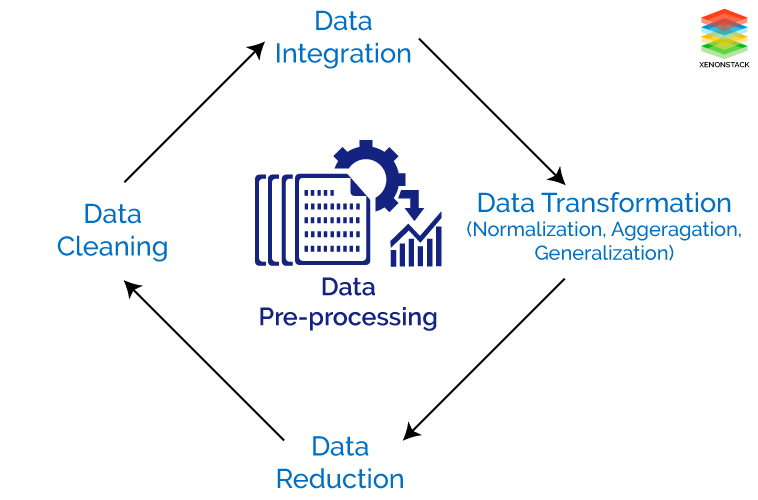
\includegraphics[width=\textwidth]{img/data-cleaning-openrefine.png}
      
\end{columns}


\begin{exampleblock}{Reconciliation}
  \begin{enumerate}\small 
      \item = alignment / matching
      \item Verbindung zu anderen Datenbanken
      \item Wikidata (en) ist automatisch dabei
      \item andere Services kann man hinzufügen:
      \begin{itemize}
          \item \href{https://tools.wmflabs.org/openrefine-wikidata/de/api}{Wikidata German}
          \item \href{https://lobid.org/gnd/reconcile}{GND}
          \item \href{https://github.com/OpenRefine/OpenRefine/wiki/Reconcilable-Data-Sources}{Ressourcenliste}
          \item \href{https://reconciliation-api.github.io/testbench/}{Testbench}
          \item \href{http://refine.codefork.com/}{Refine Codefork}
      \end{itemize}
  \end{enumerate}
\end{exampleblock}

\end{frame}


%------------------------------------------------------------------------------
\begin{frame}{Ressourcen zu OpenRefine}
\footnotesize
\metroset{block=fill}
\begin{columns}
\column{0.55\textwidth}

\begin{block}{Generelle Tutorials}
  \begin{enumerate}\scriptsize
    \item Offizielle Seite: \protect\url{http://openrefine.org/} (Links zu kurzen Youtube-Videos); textbasierte Tutorials außerdem im \href{https://docs.openrefine.org/}{User Manual}, auch Infos zur Installation, etc. Weiterhin die \href{https://github.com/OpenRefine/OpenRefine/wiki/External-Resources}{curated tutorials list} (unterschiedliche Sprachen).
    \item \href{https://github.com/OpenRefine/OpenRefine/wiki/Recipes}{OpenRefine Recipes} (vorgefertigte Lösungen für typische Probleme)
    \item \href{https://librarycarpentry.org/lc-open-refine/01-introduction/index.html}{Library Carpentry Tutorial}
    \item \href{https://data-lessons.github.io/dh-openrefine/01-introduction/}{Data Lessons `OpenRefine for Digital Humanities' Tutorial}
    \item \href{https://multimedia.journalism.berkeley.edu/tutorials/openrefine/}{Berkeley Tutorial}
    \item \href{https://studentwork.prattsi.org/dh/2016/05/07/introduction-to-openrefine/}{Digital Humanities at Pratt: Introduction to Open Refine}; dazu ein sehr gutes 30min \href{https://www.youtube.com/watch?v=WCRexQXYFrI}{Youtube-Video}.
    \item \href{https://datacarpentry.org/openrefine-socialsci/}{Data Carpentry: OpenRefine for Social Science Data}
    \item \href{https://histhub.ch/reconciling/}{Reconciling with Open Refine}
\end{enumerate}
\end{block}


\column{0.45\textwidth}

\begin{exampleblock}{Daten bereinigen}
  \begin{enumerate}\scriptsize
    \item \href{https://programminghistorian.org/en/lessons/cleaning-data-with-openrefine}{Programming Historian's \emph{Cleaning data with OpenRefine} Tutorial} = Basistutorial zum Bereinigen
    \item \href{https://thomaspadilla.org/dataprep/}{Thomas Padilla OpenRefine Tutorial} (relativ kurz)
    \item \texttt{.zip}-Dokument mit weiteren Folien und Übung
\end{enumerate}
\end{exampleblock}

\begin{alertblock}{Web Scraping}
  \begin{enumerate}\scriptsize
    \item \href{https://programminghistorian.org/en/lessons/fetch-and-parse-data-with-openrefine}{Programming Historian's \emph{Fetch and Parse Data with OpenRefine} Tutorial} = Fortgeschrittenes Tutorial um Daten aus dem Web zu ziehen (z.B. von Wikipedia)
    \item \href{https://www.youtube.com/watch?v=Wtbiv7yudtA}{Web Scraping Workshop mit Dr. Frederik Elwert}: Schnelleinstieg in HTML/Webseiten, daraufhin Web Scraping von Daten mit OpenRefine (einfacher Einstieg) 
  \end{enumerate}
\end{alertblock}

\end{columns}
    
\end{frame}


%------------------------------------------------------------------------------
\begin{frame}[standout]
    \alert{Messy Data}-Praxisübung: \\
    \begin{enumerate}
        \item Auf \protect\url{https://openrefine.org/} die kurzen Einleitunsvideos schauen (7+8+6 = 21min) und OpenRefine installieren.
        \item Das \alert{\href{https://blog.lobid.org/2018/08/27/openrefine.html}{GND reconciliation for OpenRefine}} Tutorial machen.
    \end{enumerate} 
\end{frame}

%

%------------------------------------------------------------------------------

%------------------------------------------------------------------------------

%------------------------------------------------------------------------------